\documentclass[12pt]{book}
\usepackage[margin=.85in]{geometry} % for MARGIN
\usepackage[many]{tcolorbox}    	% for COLORED BOXES (tikz and xcolor included)


\usepackage{multicol}   
\usepackage{enumerate}
\usepackage[shortlabels]{enumitem}
\usepackage{varwidth}
\usepackage{tasks}
\usepackage[export]{adjustbox}

\usepackage{titleps}
\usepackage{setspace}               % for LINE SPACING
\usepackage[⟨options⟩]{fancyhdr}
\usepackage{enumitem}
\setlist{nosep}
\usepackage{tikz}
\usepackage{pgfplots}
\pgfplotsset{compat=1.5.1}
\usetikzlibrary{datavisualization}
\usetikzlibrary{datavisualization.formats.functions}

\newcommand{\D}{\displaystyle}


\setlength\parindent{0pt}   % killing indentation for all the text
\setstretch{1.3}            % setting line spacing to 1.3
\setlength\columnsep{0.25in} % setting length of column separator
\pagestyle{fancy}           % setting pagestyle to be headings

\usepackage[]{titlesec}

\fancyhead[L]{Math V04 - College Algebra}
\fancyhead[R]{Christina Papazacharioudakis}

\tcbset{
    sharp corners,
    colback = white,
    before skip = 0.2cm,    % add extra space before the box
    after skip = 0.5cm      % add extra space after the box
}                           % setting global options for tcolorbox

    \newtcolorbox{boxR}{
    fontupper = \color{black}, % font color
    boxrule = 1.5pt,
    colframe = black,
    rounded corners,
    arc = 5pt   % corners roundness
}

\definecolor{ballblue}{rgb}{0.13, 0.67, 0.8}

\begin{document}



\begin{comment}
Name: \underline{\hspace{100mm}}
\vspace{20mm}
  \centerline{\Large \textbf{Chapter 2: Equations and Inequalities} } 

{\large
\begin{center}
\begin{varwidth}{\textwidth}
\begin{enumerate}[2.1]
    \item The Regular Coordinate System and Graphs
    \item Linear Equations in One Variable
    \item Models and  Applications (Skipping)
    \item Complex Numbers
    \item Quadratic Equations
    \item Other Types of Equations
    \item Linear Inequalities and Absolute Value Inequalities
\end{enumerate}
\end{varwidth}
\end{center}

}
\newpage  
\end{comment}

{\Large \textbf{6.6 Exponential and Logarithmic Equations}}

We now apply everything we have learned in this chapter to solve exponential and logarithmic equations! 

\vspace{2mm}

{\large \textbf{Exponential Equations}}

An \textbf{exponential equation} is an equation containing a variable in an exponent. Here are some examples,


    $$\D 2^{3x-8}=16  \hspace{15mm} 4^x = 15 \hspace{15mm} 40e^{0.6x}=240$$

Some exponential equations can be solved by expressing each side of the equation as a power of the same base. For example, looking at $2^{3x-8}=16$:


\vspace{100mm}


\centerline{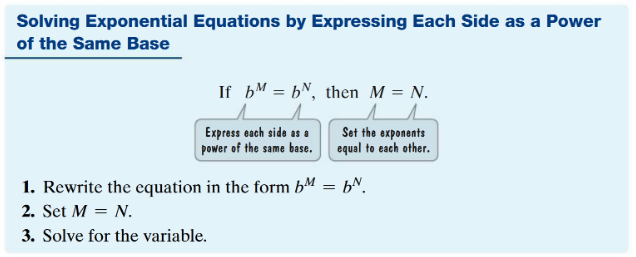
\includegraphics[scale=.6]{Chapter 6/6.7-figure1.png}}
\newpage

\underline{\textbf{Example 1 - Solving an Exponential Equation}}
\vspace{1mm}

Solve $\D 27^{x+3}=9^{x-1}$

\vspace{110mm}

Most exponential equations cannot be rewritten so that each side has the same base. Some examples: 

$$ 4^x=15 \hspace{30mm} 10^x = 120,000$$

\vspace{45mm}

Logarithms are extremely useful in solving these equations since they help us ``bring" down the variable in the exponent. Let's take a look how logarithms help us...

\newpage
\centerline{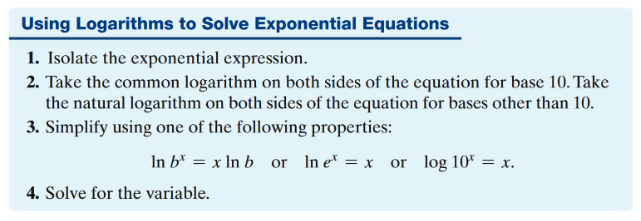
\includegraphics[scale=0.6]{Chapter 6/6.7-figure2.png}}

\underline{\textbf{Example 2 - Solving Exponential Equations with Logarithms}}

Solve: 
\begin{multicols}{3}
    \begin{enumerate}[(a)]
    \item $\D 4^x = 15$
    \item $\D 10^x=120,000$
    \item  $\D 40e^{0.6x} -3 = 237$
\end{enumerate}
\end{multicols}




\newpage
Now we look at an example where each side of the equation has an exponential equation isolated to one side. 
\vspace{5mm}

\underline{\textbf{Example 3 - Solving an Exponential Equation}}
\vspace{1mm}

Solve $\D 5^{x-2}=4^{2x+3}$


\vspace{120mm}






{\large \textbf{Logarithmic Equations}}
\vspace{3mm}

A \textbf{logarithmic equation} is an equation containing a variable in a logarithmic expression. 

Examples include,

$$ \log_4(x+3)=2 \hspace{5mm} \text{ and } \hspace{5mm} \ln(x+2)-\ln(4x+3)= \ln\left(\frac{1}{x}\right)$$

In some cases, we can rewrite the logarithmic equation into the form $\log_b(M)=c$ using the logarithmic rules we have learned. 

This form will allow us to solve equations by rewriting them in exponential form. 
\newpage

\centerline{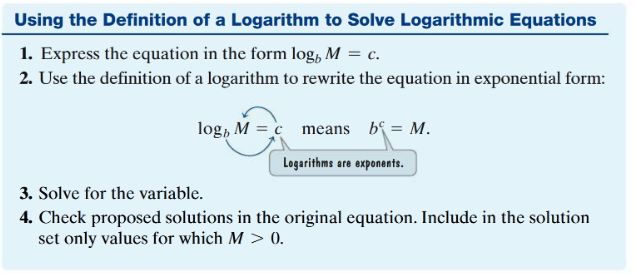
\includegraphics[scale=.6]{Chapter 6/6.7-figure3.png}}
\vspace{3mm}

\underline{\textbf{Example 4 - Solving an Exponential Equation}}
\vspace{1mm}

Solve:
\begin{multicols}{2}
    \begin{enumerate}[(a)]
    \item $\D \log_4(x+3)=2$
    \item $\D 3 \ln(2x)=12$
\end{enumerate}

\end{multicols}


\newpage
Sometimes it takes a bit more work to get the form $\log_b(M)=c$. We use logarithmic rules we learned in the previous chapter to ``condense" the equation. 

\vspace{1mm}

\underline{\textbf{Example 5 - Solving an Exponential Equation}}
\vspace{1mm}

Solve: $\D \log_2x+\log_2(x-7)=3$



\vspace{140mm}

So far we have looked at solving logarithmic equations of the form $\D \log_b(M)=c$. 

We now look at solving equations when we see logarithmic expressions appearing on both sides: 

$$\log_b(M)=\log_b(N)$$

Since logarithmic functions are one-to-one (each output comes from exactly one input), we also have $M=N$.

\newpage
\centerline{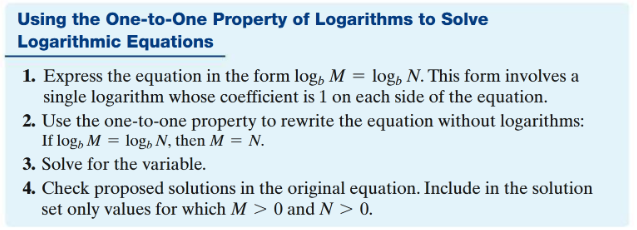
\includegraphics[scale=.7]{Chapter 6/6.7-figure4.png}}
\vspace{3mm}

\underline{\textbf{Example 6 - Solving an Exponential Equation}}
\vspace{1mm}

Solve: $\D \ln(x+2) - \ln(4x+3)= \ln\left(\frac{1}{x}\right)$





\end{document}


